\documentclass{article}

% Document extensibility %
%
% Disables native paragraph indentation
\usepackage{parskip} 
%
% Provides further bullet options for lists
\usepackage{enumitem}

% Mathematical symbol and statement packages %
%
% Necessary
\usepackage{amsmath}
\usepackage{amssymb}
%
% Extensive fraction notation
\usepackage{xfrac}
%
% Generic mathematical commands
% Notable: \degree, \celcius
\usepackage{gensymb}
%
% Variable vector notation (arrow above variable)
\usepackage{esvect}
%
% Multiline boxed equations
\usepackage{empheq}
%
% SI Unit
\usepackage{siunitx}
\usepackage{physunits}
%
% More intuitive arrays/matrices
\usepackage{array}
%
% Linear Equations
\usepackage{systeme}
%
% Boxes!
\usepackage{mdframed}

% Graphic packages %
%
% Diagrams and illustrations
\usepackage{tikz}
\usetikzlibrary{positioning}
%
% Image insertion
\usepackage{graphicx}
\graphicspath{ {./} }

% Document content %
%
% Change title of table of contents
% \renewcommand{\contentsname}{Title}

\title{Homework 7 - Energy}
\author{Corey Mostero - 2566652}
\date{9 May 2023}

\begin{document}

% Command `\hr` to insert horizontal rules
\newcommand{\hr}{\par\noindent\rule{\textwidth}{0.4pt}}

% Command to box and center math equations
\newcommand{\bc}[1]{
	\begin{equation*}
		\begin{boxed}
			{#1}
		\end{boxed}
	\end{equation*}
}

% Command for single line equations with a condition
\newcommand{\cond}[2]{
	\ifmmode
		{#1} \quad {#2}
	\else
		$$ {#1} \quad {#2} $$
	\fi
}

\maketitle
\newpage

\tableofcontents

\section{Book}

\subsection{6.19}

\begin{align*}
	m_\text{asteroid} & = \SI{2.4e15}{\kilogram} \\
	v_\text{asteroid} & = \SI{20}{\kilo \meter \per \second} = \SI{2e4}{\meter \per \second}
\end{align*}
\begin{enumerate}[label = \textbf{(\alph*)}]
	\item How much kinetic energy did this meteor deliver to the ground?
		\begin{align*}
			E & = \frac{1}{2}mv^2 \\
			E & = \frac{1}{2}(\SI{2.4e15}{\kilogram})(\SI{2e4}{\meter \per \second})^2 \\
			E & = \SI{4.8e23}{\kilogram \meter \per \second}
		\end{align*}
		\bc{ E = \SI{4.8e23}{\joule} }
	\item How does this energy compare to the energy released by a \SI{1.0}{\mega \tonne} nuclear bomb?
		\begin{align*}
			E_\text{asteroid} & = \SI{4.8e23}{\joule} \\
			E_\text{bomb} & = \SI{4.184e15}{\joule}
		\end{align*}
		\begin{align*}
			\frac{E_\text{asteroid}}{E_\text{bomb}} & \\
			\frac{\SI{4.8e23}{\joule}}{\SI{4.184e15}{\joule}} & = \SI{1.147e8}{\joule}
		\end{align*}
		\begin{mdframed}
			The kinetic energy of the asteroid is $ \SI{1.147e8}{\joule} $ as much kinetic energy from a \SI{1.0}{\mega \tonne} nuclear bomb.
		\end{mdframed}
\end{enumerate}

\subsection{6.29}

\begin{align*}
	E_A & = \SI{27}{\joule} \\
	m_B & = \frac{1}{4}E_A
\end{align*}
\begin{enumerate}[label = \textbf{(\alph*)}]
	\item If object $ B $ also has $ \SI{27}{\joule} $ of kinetic energy, is it moving faster or slower than object $ A $? By what factor?
		\begin{align*}
			E_A & = \SI{27}{\joule}
		\end{align*}
		\begin{align*}
			E_A & = E_B \\
			\frac{1}{2}m_Av_A^2 & = \frac{1}{2}m_Bv_B^2 \\
			m_Av_A^2 & = \left( \frac{1}{4}m_A \right)v_B^2 \\
			4v_A^2 & = v_B^2 \\
			v_B & = \sqrt{4v_A^2} \\
			v_B & = 2v_A
		\end{align*}
		\begin{mdframed}
			The velocity of $ v_B $ is two times $ v_A $, implying that object $ B $ is moving twice as fast as object $ A $. (The factor would be $ 2 $)
		\end{mdframed}
	\item By what factor does the speed of each object change if total work $ \SI{-18}{\joule} $ is done on each?
		\begin{align*}
			W_\text{total} & = \SI{-18}{\joule}
		\end{align*}
		\begin{align*}
			W_\text{total} & = E_A - E_B \\
			\SI{-18}{\joule} & = E_A - \SI{27}{\joule} \\
			E_A & = \SI{9}{\joule}
		\end{align*}
		\begin{align*}
			\frac{ \frac{1}{2}m_{A_f}v_{A_f}^2 }{ \frac{1}{2}m_{A_i}v_{A_i}^2 } & = \frac{E_{A_f}}{E_{B_i}} \\
			\frac{v_{A_f}^2}{v_{A_i}^2} & = \frac{\SI{9}{\joule}}{\SI{27}{\joule}} \\
			v_{A_f}^2 & = \frac{1}{3}v_{A_i}^2 \\
			v_{A_f} & = \frac{1}{\sqrt{3}}v_{A_i}
		\end{align*}
		\begin{mdframed}
		As negative work is done upon the object $ A $ calculated above, it makes sense that the resulting (final) velocity would be less than the initial velocity (in this case specifically by the factor of $ \frac{1}{\sqrt{3}} $). \\
		It can also be concluded that due to object $ A $ and $ B $ having both the same kinetic energy ($ E_A = E_B $) and work done upon them, the factor calculated will be the same.
		\end{mdframed}
\end{enumerate}

\subsection{6.31}

\begin{enumerate}[label = \textbf{(\alph*)}]
	\item Use the work-energy theorem to calculate the minimum stopping distance of the car in terms of $ v_0 $, $ g $, and the coefficient of kinetic friction $ \mu_k $ between the tires and the road. \\
		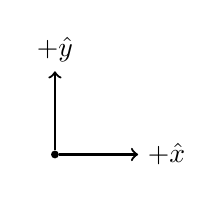
\begin{tikzpicture}
			\node[circle, fill, inner sep = 1pt] (origin) {};
			\node (y) [above = of origin] {$ +\hat{y} $};
			\node (x) [right = of origin] {$ +\hat{x} $};

			\foreach \node in {y, x}
				\draw[black, thick, ->] (origin) -- (\node);
		\end{tikzpicture}
		\begin{tikzpicture}
			\node (origin) { car };
			\node (left) [left = of origin] {$ f $};
			\node (above) [above = of origin] {$ N $};
			\node (below) [below = of origin] {$ m_\text{car}g $};

			\foreach \node in {left, above, below}
				\draw[black, thick, ->] (origin) -- (\node);
		\end{tikzpicture}
		\begin{align*}
			\sum F_y & = 0 \\
			N & = m_\text{car}g
		\end{align*}
		\begin{align*}
			W & = -fd \\
			W & = -\mu Nd \\
			W & = -\mu m_\text{car}gd
		\end{align*}
		\begin{align*}
			W & = E_f - E_i \\
			-\mu m_\text{car}gd & = 0 - \frac{1}{2}m_\text{car}v_i^2 \\
			d & = \frac{v_i^2}{2\mu g}
		\end{align*}
		\bc{ d = \frac{v_i^2}{2\mu g} }
	\item By what factor would the minimum stopping distance change if
		\begin{enumerate}[label = \textbf{(\roman*)}]
			\item \label{6.31.b.i} the coefficient of kinetic friction were doubled?
				\begin{align*}
					\mu & = 2\mu
				\end{align*}
				\begin{align*}
					W & = E_f - E_i \\
					-2\mu m_\text{car}gd_1 & = -\frac{1}{2}m_\text{car}v_i^2 \\
					d_1 & = \frac{v_i^2}{4\mu g}
				\end{align*}
				\begin{align*}
					d & : d_1 \\
					\frac{v_i^2}{2\mu g} & : \frac{v_i^2}{4\mu g} \\
					1 & : \frac{1}{2}
				\end{align*}
				\bc{\frac{1}{2}}
			\item \label{6.31.b.ii} the initial speed were doubled?
				\begin{align*}
					v_i & = 2v_i
				\end{align*}
				\begin{align*}
					W & = E_f - E_i \\
					-\mu m_\text{car}gd_1 & = -\frac{1}{2}m_\text{car}(2v_i)^2 \\
					d_1 & = \frac{2v_i^2}{\mu g}
				\end{align*}
				\begin{align*}
					d & : d_1 \\
					\frac{v_i^2}{2\mu g} & : \frac{2v_i^2}{\mu g} \\
					1 & : 4
				\end{align*}
				\bc{4}
			\item both the coefficient of kinetic friction and the initial speed were doubled? \\
				We can use parts \ref{6.31.b.i} and \ref{6.31.b.ii} to find the ratio as the $ W $ and $ E_f $ would simply expand to include the calculated values above and simplify to the expression below:
				\begin{align*}
					4 \cdot \frac{1}{2} & = 2
				\end{align*}
				\bc{2}
		\end{enumerate}
\end{enumerate}

\subsection{6.33}

\begin{align*}
	m_1 = m_2 = m_3 & = \SI{8.50}{\kilogram} \\
	k & = \SI{7.80}{\kilo \newton \per \meter} = \SI{7.80e3}{\newton \per \meter} \\
	x & = \SI{12.0}{\centi \meter}
\end{align*}

\begin{enumerate}[label = \textbf{(\alph*)}]
	\item Draw a free-body diagram of each mass. \\
		\begin{tikzpicture}
			\node[circle, fill, inner sep = 1pt] (origin) {};
			\node [below = of origin] (y) {$ +\hat{y} $};
			\node [right = of origin] (x) {$ +\hat{x} $};

			\foreach \node in {y, x}
				\draw[black, thick, ->] (origin) -- (\node);
		\end{tikzpicture}

		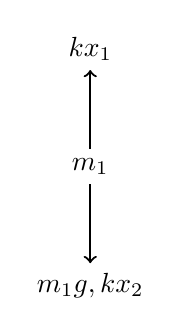
\begin{tikzpicture}
			\node (origin) {$ m_1 $};
			\node (above) [above = of origin] {$ kx_1 $};
			\node (below) [below = of origin] {$ m_1g, kx_2 $};

			\foreach \node in {above, below}
				\draw[black, thick, ->] (origin) -- (\node);
		\end{tikzpicture}
		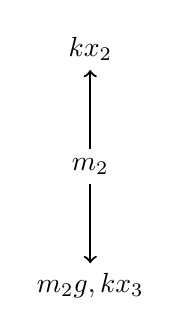
\begin{tikzpicture}
			\node (origin) {$ m_2 $};
			\node (above) [above = of origin] {$ kx_2 $};
			\node (below) [below = of origin] {$ m_2g, kx_3 $};

			\foreach \node in {above, below}
				\draw[black, thick, ->] (origin) -- (\node);
		\end{tikzpicture}
		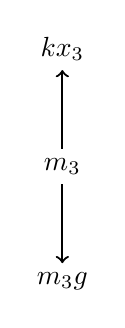
\begin{tikzpicture}
			\node (origin) {$ m_3 $};
			\node (above) [above = of origin] {$ kx_3 $};
			\node (below) [below = of origin] {$ m_3g $};

			\foreach \node in {above, below}
				\draw[black, thick, ->] (origin) -- (\node);
		\end{tikzpicture}
	\item How long is each spring when hanging as shown?
		\begin{align*}
			\sum F_y^{(m_3)} & = 0 \\
			kx_3 & = m_3g \\
			x_3 & = \frac{m_3g}{k} \\
			x_3 & = \frac{(\SI{8.50}{\kilogram})(\SI{10}{\meter \per \second \squared})}{\SI{7.80e3}{\newton \per \meter}} \\
			x_3 & = \SI{0.011}{\meter} = \SI{1.1}{\centi \meter}
		\end{align*}
		\begin{align*}
			\sum F_y^{(m_2)} & = 0 \\
			kx_2 & = m_2g + kx_3 \\
			x_2 & = \frac{m_2g + kx_3}{k} \\
			x_2 & = \frac{(\SI{8.50}{\kilogram})(\SI{10}{\meter \per \second \squared}) + (\SI{7.80e3}{\newton \per \meter})(\SI{0.011}{\meter})}{\SI{7.80e3}{\newton \per \meter}} \\
			x_2 & = \SI{0.022}{\meter} = \SI{2.2}{\centi \meter}
		\end{align*}
		\begin{align*}
			\sum F_y^{(m_1)} & = 0 \\
			kx_1 & = m_1g + kx_2 \\
			x_1 & = \frac{m_1g + kx_2}{k} \\
			x_1 & = \frac{(\SI{8.50}{\kilogram})(\SI{10}{\meter \per \second \squared}) + (\SI{7.80e3}{\newton \per \meter})(\SI{0.022}{\meter})}{\SI{7.80e3}{\newton \per \meter}} \\
			x_1 & = \SI{0.033}{\meter} = \SI{3.3}{\centi \meter}
		\end{align*}
		\begin{mdframed}
			Spring 1: $ \SI{12.0}{\centi \meter} + x_1 = \SI{15.3}{\centi \meter} $ \\
			Spring 2: $ \SI{12.0}{\centi \meter} + x_2 = \SI{14.2}{\centi \meter} $ \\
			Spring 3: $ \SI{12.0}{\centi \meter} + x_3 = \SI{13.1}{\centi \meter} $
		\end{mdframed}
\end{enumerate}

\subsection{6.45}

\begin{align*}
	F(x) & = \SI{18.0}{\newton} - (\SI{0.530}{\newton \per \meter})x \\
	m & = \SI{5.00}{\kilogram} \\
	v_0 & = 0 \\
	x_0 & = 0 \\
	x_1 & = \SI{11.0}{\meter} \\
	v_1 & = ? \\
	E_i & = 0
\end{align*}
What is its speed after it has traveled \SI{11.0}{\meter}?
\begin{align*}
	W & = \int_{x_0}^{x_1} \left( F(x) \right) dx \\
	W & = \int_{0}^{\SI{11.0}{\meter}} \left( \SI{18.0}{\newton} - (\SI{0.530}{\newton \per \meter})x \right) dx \\
	W & = \left. \left[ (\SI{18.0}{\newton})x - (\SI{0.265}{\newton \per \meter})x^2 \right] \right|_{0}^{\SI{11.0}{\meter}} \\
	W & = \left[ (\SI{18.0}{\newton})(\SI{11.0}{\meter}) - (\SI{0.265}{\newton \per \meter})(\SI{11.0}{\meter})^2 \right] - 0 \\
	W & = \SI{165.935}{\joule}
\end{align*}
\begin{align*}
	W & = E_f - E_i, & \text{$ E_i = 0 $ as $ v_0 = 0 $} \\
	W & = E_f \\
	W & = \frac{1}{2}mv_f^2 \\
	v_f & = \sqrt{ \frac{2W}{m} } \\
	v_f & = \sqrt{ \frac{2(\SI{165.935}{\joule})}{\SI{5.00}{\kilogram}} } \\
	v_f & = \SI{8.15}{\meter \per \second}
\end{align*}
\bc{ v_f = \SI{8.15}{\meter \per \second} }

\subsection{6.48}

\begin{align*}
	d & = \SI{5.0}{\kilo \meter} \\
	v_\text{run} & = \SI{10}{\kilo \meter \per \hour} \\
	P_\text{run} & = \SI{700}{\watt} \\
	v_\text{walk} & = \SI{3.0}{\kilo \meter \per \hour} \\
	P_\text{walk} & = \SI{290}{\watt}
\end{align*}
\begin{enumerate}[label = \textbf{\arabic*)}]
	\item Which choice would burn up more energy, and how much energy (in joules) would it burn?
		\begin{align*}
			d & = v_\text{run}t_\text{run} \\
			t_\text{run} & = \frac{d}{v_\text{run}} \\
			t_\text{run} & = \frac{\SI{5.0}{\kilo \meter}}{\SI{10}{\kilo \meter \per \hour}} \\
			t_\text{run} & = \SI{0.5}{\hour}
		\end{align*}
		\begin{align*}
			P & = \frac{W}{t} \\
			W_\text{run} & = P_\text{run}t_\text{run} \\
						 & = (\SI{700}{\watt})(\SI{0.5}{\hour}) \\
						 & = \SI{350}{\watt \hour} \\
			W_\text{run} & = (\SI{350}{\watt \hour}) \left( \frac{\SI{3600}{\second}}{\SI{1}{\hour}} \right) = \SI{1260000}{\joule} = \SI{1.26e6}{\joule}
		\end{align*}
		\begin{align*}
			t_\text{walk} = \frac{d}{v_\text{walk}} \\
			t_\text{walk} & = \frac{\SI{5.0}{\kilo \meter}}{\SI{3.0}{\kilo \meter \per \hour}} \\
			t_\text{walk} & = \SI{1.667}{\hour}
		\end{align*}
		\begin{align*}
			W_\text{walk} & = P_\text{walk}t_\text{walk} \\
						  & = (\SI{290}{\watt})(\SI{1.667}{\hour}) \\
						  & = \SI{483.43}{\watt \hour} \\
			W_\text{walk} & = (\SI{483.43}{\watt \hour}) \left( \frac{\SI{3600}{\second}}{\SI{1}{\hour}} \right) = \SI{1.74e6}{\joule}
		\end{align*}
		\begin{mdframed}
			Walking will take more energy than running.
		\end{mdframed}
	\item Why does the more intense exercise burn up less energy than the less intense exercise?
		\begin{mdframed}
			Because I will have to take a longer time to arrive at the physics lab by walking, it takes up more energy.
		\end{mdframed}
\end{enumerate}

\subsection{6.51}

\begin{align*}
	h & = \SI{10}{\meter} \\
	m_\text{student} & = \SI{71}{\kilogram} \\
	P & = \SI{500}{\watt} \\
	t & = ?
\end{align*}
How long would it take the student to travel up the three flights of stairs?
\begin{align*}
	P & = \frac{W}{t} \\
	t & = \frac{W}{P} \\
	t & = \frac{wh}{P} \\
	t & = \frac{(\SI{71}{\kilogram})(\SI{10}{\meter \per \second \squared})(\SI{10}{\meter})}{\SI{500}{\watt}} \\
	t & = \SI{14.2}{\second}
\end{align*}
\bc{ t = \SI{14.2}{\second} }

\subsection{7.5}

\begin{align*}
	y_0 & = \SI{20.8}{\meter} \\
	v_0 & = \SI{11.5}{\meter \per \second} \\
	\theta & = \SI{50.1}{\degree}
\end{align*}
\begin{enumerate}[label = \textbf{(\alph*)}]
	\item \label{7.5.a} What is the speed of the ball just before it strikes the ground?
		\begin{align*}
			E_0 & = E_1 \\
			\frac{1}{2}mv_0^2 + mgh_0 & = \frac{1}{2}mv_1^2 + mgh_1 \\
			v_1 & = \sqrt{ v_0^2 + 2gh_0 - gh_1 } \\
			v_1 & = \sqrt{ (\SI{11.5}{\meter \per \second}))^2 + 2(\SI{10}{\meter \per \second \squared})(\SI{20.8}{\meter}) - (\SI{10}{\meter \per \second \squared})(0) } \\
			v_1 & = \SI{23.41}{\meter \per \second}
		\end{align*}
		\bc{ v_1 = \SI{23.41}{\meter \per \second} }
	\item \label{7.5.b} What is the answer for part \ref{7.5.a} if the initial velocity is at an angle of \SI{50.1}{\degree} \textit{below} the horizontal?
		\begin{align*}
			\theta & = \SI{-50.1}{\degree}
		\end{align*}
		\begin{align*}
			v_1 & = \sqrt{ v_0^2 + 2gh_0 - gh_1 } \\
			v_1 & = \sqrt{ (\SI{11.5}{\meter \per \second}))^2 + 2(\SI{10}{\meter \per \second \squared})(\SI{20.8}{\meter}) - (\SI{10}{\meter \per \second \squared})(0) } \\
			v_1 & = \SI{23.41}{\meter \per \second}
		\end{align*}
		\bc{ v_1 = \SI{23.41}{\meter \per \second} }
	\item If the affects of air resistance are included, will part \ref{7.5.a} or \ref{7.5.b} give the higher speed?
		\begin{mdframed}
			In part \ref{7.5.b}, the tennis ball is thrown directly at the ground resulting in a shorter distance and time traveled. As the tennis ball is in the air for less time and distance, air resistance will likely have less of an overall effect when compared with throwing it above the horizontal.
		\end{mdframed}
\end{enumerate}

\subsection{7.9}

\begin{align*}
	m & = \SI{0.20}{\kilogram} \\
	v_0 & = 0 \\
	R & = \SI{0.50}{\meter} \\
	W_f & = \SI{-0.22}{\joule} \\
	y_A & = 0 \\
\end{align*}
\begin{tikzpicture}
	\node[circle, fill, inner sep = 1pt] (origin) {};
	\node [below = of origin] (y) {$ +\hat{y} $};
	\node [right = of origin] (x) {$ +\hat{x} $};

	\draw[black, thick, ->] (origin) -- (y);
	\draw[black, thick, ->] (origin) -- (x);
\end{tikzpicture}
\begin{enumerate}[label = \textbf{(\alph*)}]
	\item Between points $ A $ and $ B $, how much work is done on the rock by
		\begin{enumerate}[label = \textbf{(\roman*)}]
			\item the normal force?
				\begin{mdframed}
					$$ W_N = 0 $$
					Forces perpendicular to the displacement have 0 work done.
				\end{mdframed}
			\item gravity?
				\begin{align*}
					W_g & = E_B - E_A \\
					W_g & = mgy_B - mgy_A \\
					W_g & = (\SI{0.20}{\kilogram})(\SI{10}{\meter \per \second \squared})(\SI{0.50}{\meter}) - (\SI{0.20}{\kilogram})(\SI{10}{\meter \per \second \squared})(\SI{0}{\meter}) \\
					W_g & = \SI{1.00}{\joule}
				\end{align*}
				\bc{ W_g = \SI{1.00}{\joule} }
		\end{enumerate}
	\item What is the speed of the rock as it reaches point $ B $?
		\begin{align*}
			W & = E_B - E_A \\
			W_g - W_f & = \frac{1}{2}mv_1^2 - \frac{1}{2}mv_0^2 \\
			v_1 & = \sqrt{ 2 \left( \frac{W_g - W_f}{m} \right) } \\
			v_1 & = \sqrt{ 2 \left( \frac{\SI{1.00}{\joule} - \SI{0.22}{\joule}}{\SI{0.20}{\kilogram}} \right) } \\
			v_1 & = \SI{2.79}{\meter \per \second}
		\end{align*}
		\bc{ v_1 = \SI{2.79}{\meter \per \second} }
	\item Of the three forces acting on the rock as it slides down the bowl, which (if any) are constant and which are not? Explain.
		\begin{itemize}
			\item $ W_N $ - The work done by normal force is only zero when it is entirely orthogonal to the direction of motion, but as the rock rolls on the \textit{curve}, the angle between the direction of motion and the normal force is no longer perpendicular resulting in a \textbf{non-constant} work done by the normal force.
			\item $ W_f $ - Since the work done by $ W_N $ varies, the work done by friction varies resulting in it also being \textbf{non-constant}.
				\begin{equation*}
					W_f = F_fd\cos(\theta) = \mu Nd\cos(\theta)
				\end{equation*}
			\item $ W_g $ - As long as the mass of the rock is constant, and the rock is continuously in contact with the bowl (not falling), the work down by gravity is \textbf{constant}.
		\end{itemize}
	\item Just as the rock reaches point $ B $, what is the normal force on it due to the bottom of the bowl? \\
		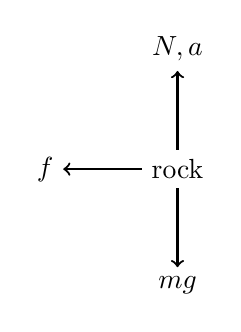
\begin{tikzpicture}
			\node (origin) {rock};
			\node [above = of origin] (above) {$ N, a $};
			\node [below = of origin] (below) {$ mg $};
			\node [left = of origin] (left) {$ f $};

			\foreach \node in {above, below, left}
				\draw[black, thick, ->] (origin) -- (\node);
		\end{tikzpicture}
		\begin{align*}
			\sum F & = -ma_{cen} \\
			mg & = N - ma_{cen} \\
			N & = mg + m \left( \frac{v_1^2}{R} \right) \\
			N & = (\SI{0.20}{\kilogram})(\SI{10}{\meter \per \second \squared}) + (\SI{0.20}{\kilogram}) \left( \frac{(\SI{2.79}{\meter \per \second})^2}{\SI{0.50}{\meter}} \right) \\
			N & = \SI{5.11}{\newton}
		\end{align*}
		\bc{ N = \SI{5.11}{\newton} }
\end{enumerate}

\subsection{7.35}

\begin{enumerate}[label = \textbf{(\alph*)}]
	\item
		\begin{align*}
			F(r) & = \frac{dU}{dr} = \frac{d}{dr} \left( \left( \frac{a}{r^{12}} \right) - \left( \frac{b}{r^6} \right) \right) \\
			F(r) & = \frac{12a}{r^{13}} - \frac{6b}{r^7}
		\end{align*}
		\begin{itemize}
			\item $$ U(r) $$
				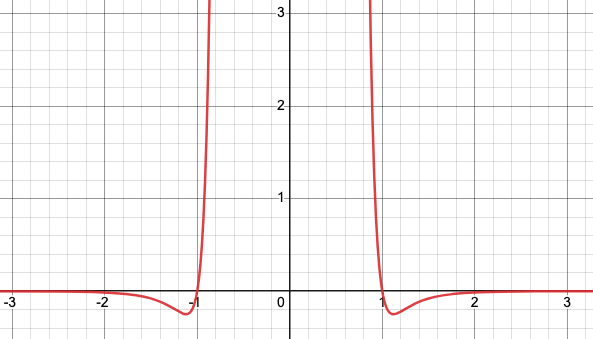
\includegraphics[width = 200pt]{graph_1.png}
			\item $$ F(r) $$
				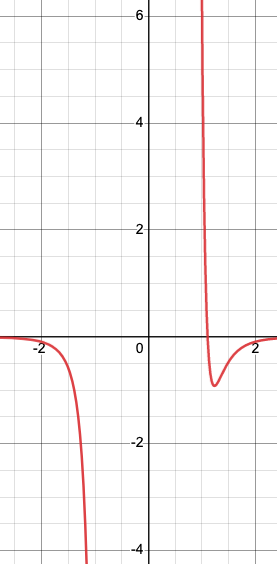
\includegraphics[width = 100pt]{graph_2.png}
		\end{itemize}
	\item Find the equilibrium distance between the two atoms. Is this equilibrium stable?
		\begin{align*}
			\frac{12a}{r^{13}} - \frac{6b}{r^7} & = 0 \\
			\frac{12a}{r^{13}} & = \frac{6b}{r^7} \\
			12a & = 6br^6 \\
			r & = \sqrt[6]{ \frac{2a}{b} }
		\end{align*}
		The equilibrium is stable.
	\item What minimum energy must be added to the molecule to \textit{dissociate} it – that is, to separate the two atoms to an infinite distance apart? \\
		\begin{align*}
			-U & = -\frac{a}{r^{12}} + \frac{b}{r^6} \\
			-U & = -\frac{a}{(\sqrt[6]{ \frac{a}{b} })^{12}} + \frac{b}{(\sqrt[6]{ \frac{a}{b} })^6} \\
			-U & = \frac{b^2}{4a}
		\end{align*}
		\bc{-U = \frac{b^2}{4a}}
	\item Find the values of the constants $ a $ and $ b $.
		\begin{align*}
			d & = \SI{1.13e-10}{\meter} \\
			E & = \SI{1.54e-18}{\joule} \\
			a & = ? \\
			b & = ?
		\end{align*}
		\begin{align*}
			r & = d \\
			\sqrt[6]{ \frac{2a}{b} } & = \SI{1.13e-10}{\meter} \\
			\frac{2a}{b} & = \SI{2.08e-60}{\meter \tothe 6} \\
			a & = (\SI{1.04e-60}{\meter \tothe 6})b
		\end{align*}
		\begin{align*}
			U & = E \\
			\frac{b^2}{4a} & = \SI{1.54e-18}{\joule} \\
			\frac{b^2}{4(\SI{1.04e-60}{\meter \tothe 6})b} & = \SI{1.54e-18}{\joule} \\
			b & = \SI{6.41e-78}{\joule \meter \tothe 6}
		\end{align*}
		\begin{align*}
			a & = (\SI{1.04e-60}{\meter \tothe 6})b \\
			a & = (\SI{1.04e-60}{\meter \tothe 6})(\SI{6.41e-78}{\joule \meter \tothe 6}) \\
			a & = \SI{6.67e-138}{\joule \meter \tothe {12}}
		\end{align*}
		\bc{ a = \SI{6.67e-138}{\joule \meter \tothe {12}}, b = \SI{6.41e-78}{\joule \meter \tothe 6} }
\end{enumerate}

\subsection{7.40}

\begin{align*}
	m & = \SI{2.00}{\kilogram} \\
	k & = \SI{400}{\newton \per \meter} \\
	x & = \SI{0.220}{\meter} \\
	\theta & = \SI{37.0}{\degree} \\
	v_1 & = ? \\
	x_1 & = ?
\end{align*}
\begin{enumerate}[label = \textbf{(\alph*)}]
	\item What is the speed of the block as it slides along the horizontal surface after having left the spring?
		\begin{align*}
			E_{spring} & = E_p \\
			\frac{1}{2}kx^2 & = \frac{1}{2}mv_1^2 \\
			v_1 & = x\sqrt{ \frac{k}{m} } \\
			v_1 & = (\SI{0.220}{\meter}) \sqrt{ \frac{\SI{400}{\newton \per \meter}}{\SI{2.00}{\kilogram}} } \\
			v_1 & = \SI{3.11}{\meter \per \second}
		\end{align*}
		\bc{ v_1 = \SI{3.11}{\meter \per \second} }
	\item How far does the block travel up the incline before starting to slide back down?
		\begin{align*}
			E_{spring} & = E_p \\
			\frac{1}{2}kx^2 & = mgd\sin(\theta) \\
			d & = \frac{kx^2}{2mg\sin(\theta)} \\
			d & = \frac{(\SI{400}{\newton \per \meter})(\SI{0.220}{\meter})}{2(\SI{2.00}{\kilogram})(\SI{10}{\meter \per \second \squared})\sin(\SI{37.0}{\degree})} \\
			d & = \SI{0.804}{\meter}
		\end{align*}
		\bc{ d = \SI{0.804}{\meter} }
\end{enumerate}

\subsection{7.58}

\begin{align*}
	\text{truck mass} & = m \\
	\text{first slope angle} & = \alpha \\
	\text{initial speed} & = v_0 \\
	\text{distance} & = L_0 \\
	\text{second slope angle} & = \beta \\
	\text{second slope coefficient of rolling friction} & = \mu_r \\
	\text{max distance up second ramp} & = L_1 = ?
\end{align*}
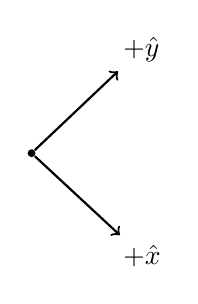
\begin{tikzpicture}
	\node[circle, fill, inner sep = 1pt] (origin) {};
	\node [above right = of origin] (y) {$ +\hat{y} $};
	\node [below right = of origin] (x) {$ +\hat{x} $};

	\foreach \node in {y, x}
		\draw[black, thick, ->] (origin) -- (\node);
\end{tikzpicture}
\begin{tikzpicture}
	\node (origin) {truck (first slope)};
	\node [above right = of origin] (above_right) {$ N $};
	\node [below = of origin] (below) {$ mg $};

	\foreach \node in {above_right, below}
		\draw[black, thick, ->] (origin) -- (\node);
\end{tikzpicture}

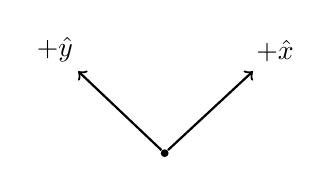
\begin{tikzpicture}
	\node[circle, fill, inner sep = 1pt] (origin) {};
	\node [above left = of origin] (y) {$ +\hat{y} $};
	\node [above right = of origin] (x) {$ +\hat{x} $};

	\foreach \node in {y, x}
		\draw[black, thick, ->] (origin) -- (\node);
\end{tikzpicture}
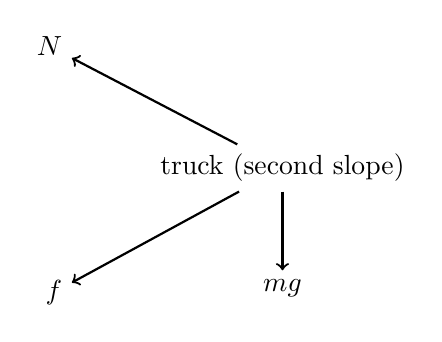
\begin{tikzpicture}
	\node (origin) {truck (second slope)};
	\node [above left = of origin] (above_left) {$ N $};
	\node [below = of origin] (below) {$ mg $};
	\node [below left = of origin] (below_left) {$ f $};

	\foreach \node in {above_left, below, below_left}
		\draw[black, thick, ->] (origin) -- (\node);
\end{tikzpicture}

Since the distance the truck halts at is being found, it can be assumed that $ v_1 = 0 $.
\begin{align*}
	E_k + E_p & = E_k + E_p - W_f \\
	\frac{1}{2}mv_0^2 + mgL_0\sin(\alpha) & = \frac{1}{2}mv_1^2 + mgL_1\sin(\beta) - \mu N \\
	\frac{1}{2}mv_0^2 + mgL_0\sin(\alpha) & = 0 + mgL_1\sin(\beta) - (-\mu_r mgL_1\cos(\beta)) \\
	L_1 & = \frac{v_0^2 + 2\sin(\alpha)gL_0}{2g(\mu \cos(\beta) + \sin(\beta))}
\end{align*}
\bc{ L_1 = \frac{v_0^2 + 2\sin(\alpha)gL_0}{2g(\mu \cos(\beta) + \sin(\beta))} }

\section{Lab Manual}

\subsection{871}

\begin{enumerate}[label = \textbf{(\alph*)}]
	\item
		\begin{align*}
			F_y & = -\frac{dU(r)}{dy} \\
			F_y & = -\frac{d}{dy} \left( mgy \right) \\
			F_y & = -mg
		\end{align*}
		The slope of the force is the weight of the object at any point $ y $.
	\item
		\begin{align*}
			U & = \int \left( kx \right) dx \\
			U & = \frac{1}{2}kx^2 + C
		\end{align*}
		``$ K $ must always be positive at all positions. Also, $ K = H - U $. Therefore, $ H - U $ must always be positive, or, in other words, $ U $ cannot ever be greater than $ H $."
		\begin{itemize}
			\item U(x) 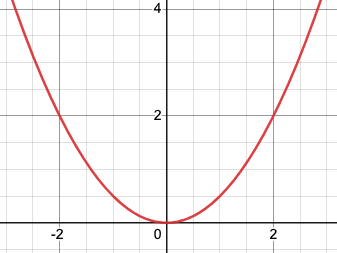
\includegraphics[width = 200pt]{graph_3.png}
			\item K(x) 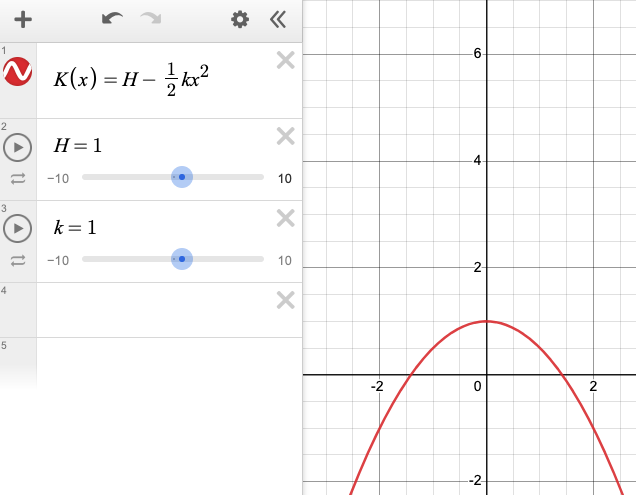
\includegraphics[width = 200pt]{graph_4.png}
		\end{itemize}
	\item \label{871.c}
		\begin{align*}
			F & = \frac{dU}{dr} = \frac{d}{dr} \left( \frac{-k}{r} \right) \\
			F & = -\frac{k}{r^2}
		\end{align*}
	\item
	\item Found in part \ref{871.c}: $$ F = -\frac{k}{r^2} $$
	\item Yes because as \textbf{Figure 3} extends to $ \infty $ it gradually attracts towards \SI{0}{ergs}
	\item
		When $ H = \sfrac{1}{2} \times 10^{-12} $, it can move between $ r_0 < r <= r_6 $. \\
		When $ H = -\sfrac{1}{2} \times 10^{-12} $, it can move between $ r_2 <= r <= r_4 $.
	\item
		A curve that approaches $ 0 $ as $ y \rightarrow \infty $.
\end{enumerate}

\subsection{876}

\begin{enumerate}[label = \textbf{(\alph*)}]
	\item
		\begin{align*}
			F_1 & = k_1x_1 \\
			x_1 & = \frac{F_1}{k_1} \\
			F_2 & = k_2x_1 \\
			x_2 & = \frac{F_2}{k_2}
		\end{align*}
		\begin{align*}
			\sum x & = x_1 + x_2 \\
			\sum F & = \sum k x \\
			x & = \frac{\sum F}{\sum k}
		\end{align*}
		\begin{align*}
			\frac{F}{k_{eq}} & = \frac{F}{k_1} + \frac{F}{k_2} \\
			\frac{1}{k_{eq}} & = \frac{1}{k_1} + \frac{1}{k_2} \\
			k_{eq} & = \frac{k_1k_2}{k_1 + k_2}
		\end{align*}
	\item
		\begin{align*}
			W & = \int_0^x k_{eq}x dx \\
			W & = \left[ \frac{1}{2}k_{eq}x^2 \right]_0^x \\
			W & = \frac{1}{2}k_{eq}x^2
		\end{align*}
		\begin{align*}
			F & = kx \\
			x & = \frac{F}{k} \\
			W & = \frac{1}{2}k_{eq} \left( \frac{F}{k} \right)^2 \\
			W & = \frac{1}{2}\frac{F^2}{k_1} + \frac{1}{2}\frac{F^2}{k_2} \\
			W & = \frac{1}{2}k_1x_1^2 + \frac{1}{2}k_2x_2^2
		\end{align*}
\end{enumerate}

\subsection{884}

\begin{align*}
	r & = \SI{4}{ft} \\
	\theta & = \SI{37}{\degree} \\
	v_0 & = 0 \\
	\mu & = 0.3
\end{align*}
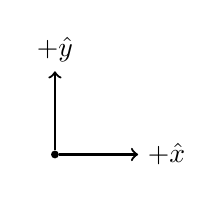
\begin{tikzpicture}
	\node[circle, fill, inner sep = 1pt] (origin) {};
	\node [above = of origin] (y) {$ +\hat{y} $};
	\node [right = of origin] (x) {$ +\hat{x} $};

	\foreach \node in {y, x}
		\draw[thick, black, ->] (origin) -- (\node);
\end{tikzpicture}
\begin{align*}
	W_{grav} + W_f & = E_1 - E_0 \\
	-mgh - \mu mg\cos(\theta)\left( \frac{h}{\sin(\theta)} \right) & = 0 - mgr \\
	h & = \frac{r}{\mu \cot(\theta) + 1} \\
	h & = \frac{\SI{4}{ft}}{(0.3)\cot(\SI{37}{\degree}) + 1} \\
	h & = \SI{2.86}{ft}
\end{align*}
\begin{align*}
	W_f & = \left( \mu mg\cos(\theta) \right) \left( \frac{h}{\sin(\theta)} \right) \\
	W_f & = \left( (0.3)\cos(\SI{37}{\degree})mg \right) \left( \frac{\SI{2.86}{ft}}{\sin(\SI{37}{\degree})} \right) \\
	W_f & = (\SI{1.14}{ft})mg
\end{align*}
\bc{ W_f = (\SI{1.14}{ft})mg }

\subsection{885}

\begin{align*}
	L & = \SI{2}{ft} \\
	\theta & = \SI{60}{\degree} \\
	y & = 0 \text{ at lowest point}
\end{align*}
\begin{enumerate}[label = \textbf{(\alph*)}]
	\item
		\begin{align*}
			E_{low} & = E_k + E_p \\
			E_{low} & = \frac{1}{2}mv_{max}^2 + mgy \\
			E_{low} & = \frac{1}{2}mv_{max}^2 + 0 \\
			E_{low} & = \frac{1}{2}mv_{max}^2
		\end{align*}
		\begin{align*}
			E_{high} & = E_k + E_p \\
			E_{high} & = \frac{1}{2}mv^2 + mgy \\
			E_{high} & = \frac{1}{2}m(0)^2 + mgy \\
			E_{high} & = mgy
		\end{align*}
		\begin{align*}
			E_{low} & = E_{high} \\
			\frac{1}{2}mv_{max}^2 & = mgy \\
			v_{max} & = \sqrt{2gy}, \quad \text{The height of the bob is non-constant, and can be found as $ L(1 - \cos(\theta)) $} \\
			v_{max} & = \sqrt{2g L(1 - \cos(\theta))}
		\end{align*}
		\begin{align*}
			v_{max} & = \sqrt{2g L(1 - \cos(\theta))} \\
			v_{max} & = \sqrt{2(\SI{32.17}{ft \per \second \squared})(\SI{2}{ft})(1 - \cos(\SI{60}{\degree}))} \\
			v_{max} & = \SI{8.02}{ft \per \second}
		\end{align*}
	\item
		\begin{align*}
			\frac{1}{2}mv_{max}^2 + mgh_0 & = \frac{1}{2}m \left( \frac{1}{2}v_{max} \right)^2 + mgL(1 - \cos(\theta)) \\
			1 - \cos(\theta) & = \frac{\frac{1}{2}v_{max}^2 - \frac{1}{2}\left(\frac{1}{2}v_{max}\right)^2}{gL} \\
			\theta & = \arccos \left( -\frac{\frac{1}{2}v_{max}^2 - \frac{1}{2}\left(\frac{1}{2}v_{max}\right)^2}{gL} + 1 \right) \\
			\theta & = \arccos \left( -\frac{\frac{1}{2}(\SI{8.02}{ft \per \second})^2 - \frac{1}{2}\left(\frac{1}{2}(\SI{8.02}{ft \per \second})\right)^2}{(\SI{32.17}{ft \per \second \squared})(\SI{2}{ft})} + 1 \right) \\
			\theta & = \SI{51.31}{\degree}
		\end{align*}
	\item
		\begin{align*}
			a & = \frac{v^2}{R} \\
			a & = \frac{(\SI{8.02}{ft \per \second})^2}{\SI{2}{ft}} \\
			a & = \SI{32.16}{ft \per \second \squared}
		\end{align*}
\end{enumerate}

\end{document}
